\begin{wrap}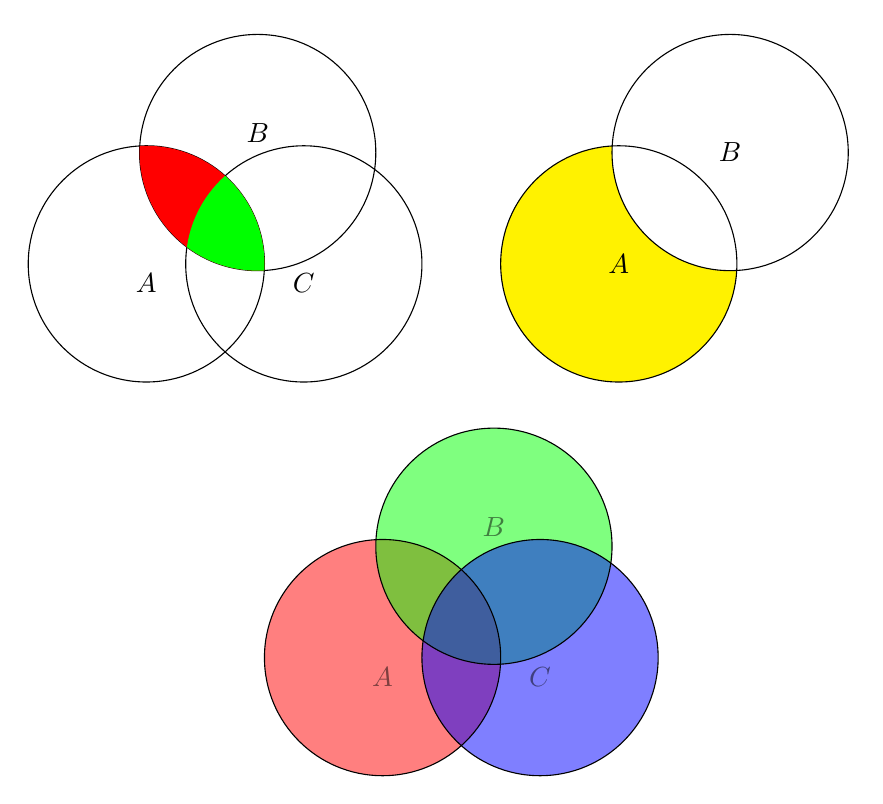
\begin{tikzpicture}
\def\firstcircle{(0,0) circle (1.5cm)}
\def\secondcircle{(45:2cm) circle (1.5cm)}
\def\thirdcircle{(0:2cm) circle (1.5cm)}

% Now we can draw the sets:
    \draw \firstcircle node[below] {$A$};
    \draw \secondcircle node [above] {$B$};
    \draw \thirdcircle node [below] {$C$};

    % Now we want to highlight the intersection of the first and the
    % second circle:

    \begin{scope}
      \clip \firstcircle;
      \fill[red] \secondcircle;
    \end{scope}

    % Next, we want the highlight the intersection of all three circles:

    \begin{scope}
      \clip \firstcircle;
      \clip \secondcircle;
      \fill[green] \thirdcircle;
    \end{scope}

    % The intersection trick works pretty well for intersections. If you need
    % the set-theoretic difference between two sets, things are a little more
    % complicated:

    % Suppose we want to highlight the part of the first circle that is not 
    % also part of the second circle. For this, we need to clip against the 
    % "complement" of the second circle. The trick is to add a large rectangle
    % that encompasses everything and then use the even-odd filling rule 
    % (see the manual again):

    \begin{scope}[shift={(6cm,0cm)}]
        \begin{scope}[even odd rule]% first circle without the second
            \clip \secondcircle (-3,-3) rectangle (3,3);
        \fill[yellow] \firstcircle;
        \end{scope}
        \draw \firstcircle node {$A$};
        \draw \secondcircle node {$B$};
    \end{scope}
    
    % When using the above, you will notice that the border lines of the
    % original circles are erased by the intersection parts. To solve this
    % problem, either use a background layer (see the manual) or simply draw
    % the border lines after everything else has been drawn.
    
    % The last trick is to cheat and use transparency
    \begin{scope}[shift={(3cm,-5cm)}, fill opacity=0.5]
        \fill[red] \firstcircle;
        \fill[green] \secondcircle;
        \fill[blue] \thirdcircle;
        \draw \firstcircle node[below] {$A$};
        \draw \secondcircle node [above] {$B$};
        \draw \thirdcircle node [below] {$C$};
    \end{scope}

\end{tikzpicture}\end{wrap}
